\documentclass{article}

% Practical-work report, not a conference submission: "preprint" shows the author and no NeurIPS claim.
\usepackage[preprint]{neurips_2026}

\usepackage[utf8]{inputenc}
\usepackage[T1]{fontenc}
\usepackage{hyperref}
\usepackage{url}
\usepackage{booktabs}
\usepackage{amsfonts}
\usepackage{amsmath}
\usepackage{nicefrac}
\usepackage{microtype}
\usepackage{xcolor}
\usepackage{graphicx}
\usepackage{tabularx}
\usepackage{caption}
\usepackage{enumitem}
\usepackage{courier}

\definecolor{linkblue}{HTML}{1F5A85}
\hypersetup{colorlinks=true,linkcolor=linkblue,citecolor=linkblue,urlcolor=linkblue}

\newcommand{\repo}{https://github.com/OMAR622-ai/dna-xlstm-charna}
\newcommand{\notebook}{\repo/blob/charna-gbst/notebooks/GBST_BERT_full_pipeline.ipynb}

\title{Does a Learned Tokenizer Help a Small DNA Language Model?\\ GBST-BERT on the Human Genome}

\author{
  Omar Mohamed (K12103822)\\
  Practical Work, Institute for Machine Learning\\
  Johannes Kepler University Linz, Austria\\
  Supervisor: Dr.\ Sohvi Luukkonen
}

\begin{document}

\maketitle

\begin{abstract}
DNA language models must decide how to cut a sequence into units before they can learn from it, and
most fix this choice in advance: one token per base, or k-mers of a set length. ChaRNABERT showed
for RNA that a learned tokenizer, Gradient-Based Subword Tokenization (GBST), can replace this choice:
at every position it builds candidate blocks of several lengths and learns how much weight each one
receives. We ask whether this idea transfers to DNA at the small scale of DNA-xLSTM. We implement
the architecture in the DNA-xLSTM code base and pretrain a 2.1M-parameter model, GBST-BERT, by
masked language modelling on the human genome (hg38) under the short-context protocol of Bio-xLSTM
(10,000 steps, 10.5B bases), next to a Transformer++ control of the same shape. We then fine-tune
both models on the 18 Nucleotide Transformer tasks with 10 seeds each and compare them with the
values published for Bio-xLSTM's models. Pretraining does not separate the two models (test
accuracy on masked bases 56.44\% vs.\ 56.33\%). Downstream, GBST-BERT has the best mean of seven
models on 13 tasks and exceeds the control on 16 of 18, with the largest gains on histone marks and
splice sites; it is weakest on enhancers. GBST places 98\% of its weight on single bases, so it
does not learn multi-base units on human DNA. We suspect the gain comes from its convolution, but
the control also differs in normalization and learning-rate tuning, so this remains to be tested
with an ablation. Finally, we show that the weak enhancer scores coincide with a train--test
mismatch in the benchmark itself: a plain 4-mer classifier shows the same drop from validation to
test, and a quarter of the test sequences are exact copies of training sequences. Code, trained
models and an executed notebook that reproduces every table are public.
\end{abstract}

\section*{Ten questions and answers}

\begin{description}[leftmargin=0pt,itemsep=3pt,topsep=2pt]
  \item[1. What question does this work ask?] Whether a learned tokenizer helps a small DNA language
  model, compared with reading one base at a time, at the 2M-parameter scale of DNA-xLSTM.

  \item[2. What is GBST, and why try it on DNA?] GBST builds candidate blocks of 1 to 4 bases around
  each position and learns how much weight each one receives. Functional DNA units have varied
  lengths, from CpG pairs to codons and motifs, so a model that chooses its own units is attractive
  (Section~\ref{sec:intro}).

  \item[3. What was built?] GBST-BERT: GBST followed by a bidirectional 4-block Transformer encoder,
  2,107,392 parameters, added to the DNA-xLSTM code base. It comes with 26 automated tests, a one-file
  version of the model and a notebook covering the whole pipeline (Section~\ref{sec:method}).

  \item[4. How was it trained?] By masked language modelling on hg38, with the short-context protocol
  of Bio-xLSTM: 10,000 steps of $2^{20}$ bases, 10.5B bases in total (Section~\ref{sec:setup}).

  \item[5. How was it evaluated?] On masked-base prediction, and on the 18 Nucleotide Transformer tasks
  (10 seeds), next to a Transformer++ control and the
  values published in Bio-xLSTM. No choice was made on test data.

  \item[6. What is the main result?] Pretraining is a tie (56.44\% vs.\ 56.33\%). On the NT tasks
  GBST-BERT has the best mean of seven models on 13 of 18 and exceeds its control on 16 of 18.

  \item[7. Did GBST learn DNA ``words''?] No. The final model places 98\% of its weight on single
  bases, so it does not form multi-base units on human DNA in this setup (Section~\ref{sec:gbstres}).

  \item[8. Does this prove that the tokenizer causes the gain?] No. The control also differs in
  normalization and in how its learning rate was chosen, and each model was pretrained once. We
  suspect GBST's convolution, but that is untested; replacing GBST with an embedding table in the same
  model would settle it (Section~\ref{sec:disc}).

  \item[9. Why are enhancers the weakest tasks?] Both enhancer tasks score far lower on test than on
  validation, unlike the other 16 tasks, and a plain 4-mer classifier shows the same drop. This points
  to a train--test mismatch in the dataset. A quarter of the test sequences are also exact copies of
  training sequences (Section~\ref{sec:enh}).

  \item[10. Can the results be reproduced, and what comes next?] The notebook re-computes all tables
  and figures from the saved runs and repeats one fine-tuning job; switches repeat the
  long runs. The next steps are the ablation in question 8 and repeated pretraining with other seeds.
\end{description}

\section{Introduction}\label{sec:intro}

Genomes are long texts over a four-letter alphabet, and language models trained on them have become
a general tool for predicting regulatory and functional properties of DNA
\citep{dallatorre2023nt,nguyen2023hyenadna,schiff2024caduceus}. Such models are first
pretrained on unlabelled genomes, usually by hiding some bases and asking the model to recover them,
and then fine-tuned on small labelled datasets, for example to recognise promoters, enhancers,
splice sites or regions carrying a given histone modification. This two-step approach is attractive
for biology because labelled data are scarce and expensive, while genome sequence is abundant.
Before such a model can learn anything, however, it must decide how to cut its input into units,
and for DNA this choice is not obvious.
Natural language offers words as a starting point; DNA has no spaces, and its functional units have
very different lengths and meanings. A methylation site involves two bases, a codon three, and a
transcription-factor binding site typically six to ten; splice sites depend on short dinucleotides
in a wider context, and the same sequence can matter in one region and not in another.

\textbf{Fixed tokenizations have known trade-offs.} One token per base keeps single-nucleotide
resolution, which matters for variants, and is used by HyenaDNA, Caduceus and DNA-xLSTM, but it leaves
all grouping of bases to the network. K-mers, as in the Nucleotide Transformer, shorten the sequence,
but they fix the unit length in advance, and a single base change or shift alters every token that
overlaps it, so that the same motif can look different depending on where it falls relative to token
boundaries. In both cases the unit is chosen by the modeller before seeing the data.

\textbf{A learned alternative.} GBST \citep{tay2022charformer} makes this choice part of training. At
each position it forms candidate blocks of several sizes and learns how much weight each deserves, so
that gradients shape the tokenization together with the rest of the network. ChaRNABERT
\citep{moralespastor2024charnabert} removed GBST's downsampling step to keep one output per
character, combined it with a bidirectional encoder, and trained RNA models of 8M to 650M parameters
on 62 million sequences. It reports a lower loss than single-character input in most settings, for
example 0.498 vs.\ 0.508 for its 5M model. If such a module also helps on DNA, it would be a cheap
addition: in our model it accounts for 3.3\% of the parameters.

\textbf{Why the small-model setting.} DNA-xLSTM \citep{schmidinger2024bioxlstm} shows that 2M-parameter
models can be strong on DNA, and it publishes a complete protocol: data, training budget, fine-tuning
procedure, and scores of several architectures. This gives a fixed reference. A small model is also
where a good inductive bias should matter most, and where repeated fine-tuning remains affordable on
shared GPUs.

\textbf{Why a controlled comparison is needed.} Published DNA models differ in many ways at once:
size, architecture, training data, number of training steps and fine-tuning budget. When one of them
scores higher, it is rarely clear which difference is responsible. To isolate the input module we
keep everything else as fixed as possible: GBST-BERT and Transformer++ have the same encoder width
and depth, nearly the same number of parameters (2.11M vs.\ 2.04M), the same pretraining data and
budget, and the same fine-tuning protocol. Comparing with Bio-xLSTM's published values then places
both models among other architectures of the same size, trained under the same protocol.

\textbf{What this report does.} We implement GBST-BERT inside the DNA-xLSTM code base, so that it
uses the same data pipeline, training loop and evaluation scripts as the published models, and test
it against a separate implementation of ChaRNABERT's equations. We pretrain both models on hg38 and
fine-tune them on 18 tasks with 10 seeds each, giving 384 fine-tuning runs. We then look inside the
model to see which block sizes GBST uses, and we examine the weakest result, the enhancer tasks, with
a simple baseline that needs no neural network. All runs, code and trained models are public, and a
notebook re-computes every table and figure from the saved runs.

\textbf{Research questions.} We keep ChaRNABERT's architecture and change the data, and we ask:
\begin{enumerate}
  \item[\textbf{RQ1.}] Does GBST improve masked-base prediction on the human genome?
  \item[\textbf{RQ2.}] Does it improve downstream prediction, relative to a same-shape control and to
  published models of similar size?
  \item[\textbf{RQ3.}] What does GBST learn on DNA: does it form multi-base units?
\end{enumerate}

\textbf{Contributions.}
\begin{itemize}
  \item An implementation of GBST-BERT in the DNA-xLSTM code base, tested against a reference
  implementation of the published equations, and released with a one-file model and a notebook.
  \item A comparison with Transformer++ in pretraining and on 18 downstream tasks (384 fine-tuning
  runs), reported with all repeats.
  \item An analysis of what GBST learned on DNA, which differs from the motivation for using it.
  \item A diagnosis of the two NT enhancer tasks, which affects how these tasks should be read.
\end{itemize}

\textbf{Summary of findings.} The answer to RQ1 is no: after 10.5B bases both models predict masked
bases equally well (56.44\% vs.\ 56.33\%). The answer to RQ2 is a qualified yes: GBST-BERT has the
best mean of seven models on 13 of 18 tasks and exceeds the control on 16 (sign test $p=0.0013$),
with gains of up to $+0.190$ MCC on histone marks, but it is clearly behind the best published model
on enhancers (MCC 0.336 vs.\ 0.546). The answer to RQ3 is unexpected: GBST puts 98\% of its weight
on single bases, so the tokenizer does not do what motivated it. Because the control is not an exact
copy of GBST-BERT without GBST, these results show that GBST-BERT is a strong small DNA model, but
not yet that the tokenizer causes its advantage.

Section~\ref{sec:background} gives background, Section~\ref{sec:method} the method,
Section~\ref{sec:setup} the data and protocols, Section~\ref{sec:results} the results, and
Section~\ref{sec:disc} what they do and do not support.

\section{Background}\label{sec:background}

\textbf{Tokenization of biological sequences.} Bio-xLSTM and Caduceus \citep{schiff2024caduceus} use
one token per base, as does HyenaDNA \citep{nguyen2023hyenadna}; the Nucleotide Transformer
\citep{dallatorre2023nt} uses k-mers. GBST \citep{tay2022charformer} forms candidate blocks of
characters and lets a scoring network weight them, which makes the tokenization differentiable.
ChaRNABERT removes Charformer's downsampling, so that one output per character remains.

\textbf{Evaluation.} Bio-xLSTM evaluates DNA models of 2M parameters on the 18 Nucleotide Transformer
(NT) tasks. We reuse its reported values as references.

\section{Method}\label{sec:method}

The model has three parts: GBST, a bidirectional encoder and a task head. Only GBST distinguishes
it from a standard character-level encoder.

\subsection{Input}

A sequence is a list of $L$ tokens $x_1,\dots,x_L$ with one token per base (A\,=\,7, C\,=\,8, G\,=\,9,
T\,=\,10, N\,=\,11; 0--6 are special tokens such as \texttt{[MASK]} and \texttt{[PAD]}), using the
repository's character tokenizer. The vocabulary has 12 entries. All candidate blocks are built
inside the model, so no tokenizer needs to be trained separately.

\subsection{GBST}\label{sec:gbst}

GBST maps the tokens to one vector per position, $z_1,\dots,z_L\in\mathbb{R}^{d}$ with $d=256$, in
five steps.

\textbf{(1) Local mixing.} Each token is embedded, passed through a depthwise convolution of width
$M=4$ (one filter per dimension, padded to keep the length), and then through a pointwise linear layer:
\begin{equation}
  u = \mathrm{Pointwise}\big(\mathrm{DWConv}_M(E[x_1],\dots,E[x_L])\big).
\end{equation}
After this step, each position already holds information about its neighbours.

\textbf{(2) Candidate blocks.} For every block size $b\in\{1,\dots,M\}$ and offset $o\in\{0,\dots,b-1\}$,
position $i$ receives the block that starts $o$ positions before it, pooled by a sum:
\begin{equation}
  B_{i,(b,o)} = \sum_{j=i-o}^{i-o+b-1} u_j ,
\end{equation}
where positions outside the sequence contribute zero. This gives $K=\sum_{b=1}^{M} b=10$ candidates per
position, all containing position $i$ (Table~\ref{tab:cand}). Offsets act like reading frames.

\begin{table}[h]
  \caption{The 10 GBST candidates for position 3 (the first T, counting from 0) of \texttt{ACGTTGCA}.}
  \label{tab:cand}
  \centering
  \small
  \begin{tabular}{cl}
    \toprule
    Block size & Candidate blocks containing position 3 \\
    \midrule
    1 & \texttt{T} \\
    2 & \texttt{TT}, \texttt{GT} \\
    3 & \texttt{TTG}, \texttt{GTT}, \texttt{CGT} \\
    4 & \texttt{TTGC}, \texttt{GTTG}, \texttt{CGTT}, \texttt{ACGT} \\
    \bottomrule
  \end{tabular}
\end{table}

\textbf{(3) Scoring.} A linear scorer $w\in\mathbb{R}^d$ rates every candidate, and a softmax over the
$K$ candidates gives weights $P\in\mathbb{R}^{L\times K}$:
\begin{equation}
  P_{i,k} = \frac{\exp(w^\top B_{i,k})}{\sum_{k'}\exp(w^\top B_{i,k'})}.
\end{equation}

\textbf{(4) Calibration.} Following ChaRNABERT (its Eq.~6), positions with similar weight patterns are
pulled towards each other:
\begin{equation}
  \hat P = \mathrm{softmax}\big(PP^\top\big)\,P ,
\end{equation}
with the softmax taken over rows. This step costs $O(L^2K)$, which is modest at $L=1{,}024$.

\textbf{(5) Mixing.} Position $i$ receives the weighted sum of its candidates,
$z_i=\sum_{k}\hat P_{i,k}\,B_{i,k}$. As in ChaRNABERT there is no downsampling, so the output has one
vector per base and the encoder sees the full sequence length.

GBST has 70,144 parameters: embedding 3,072, convolution 1,280, pointwise layer 65,536, scorer 256.
The pointwise layer is not in ChaRNABERT's equations; we infer it from the paper's parameter table,
which counts $d\cdot M+d^2$ weights for this stage. We set $M=4$ ourselves, as the paper does not state the maximum block size.

\subsection{Encoder and pretraining objective}

The encoder is a stack of 4 pre-norm blocks with bidirectional attention:
\begin{equation}
  h' = h + \mathrm{Attn}(\mathrm{LN}(h)),\qquad h_{\text{next}} = h' + \mathrm{SwiGLU}(\mathrm{LN}(h')).
\end{equation}
Attention uses 8 heads, rotary position embeddings \citep{su2024roformer} and LayerNorm on queries
and keys (QK normalization). The feed-forward layer is SwiGLU \citep{shazeer2020glu} with hidden size
320. All norms and linear layers have no bias. A final LayerNorm and a linear head give a score for
each vocabulary entry at each position. The whole model has 2,107,392 parameters.

Pretraining uses masked language modelling \citep{devlin2019bert}. A set $\mathcal{M}$ of 15\% of the
positions is selected; of these, 80\% are replaced by \texttt{[MASK]}, 10\% by a random token, and 10\%
stay unchanged. With $\tilde x$ the corrupted sequence, the loss is the mean cross-entropy over the selected
positions,
\begin{equation}
  \mathcal{L} = -\frac{1}{|\mathcal{M}|}\sum_{i\in\mathcal{M}} \log p_\theta(x_i\mid\tilde x),
\end{equation}
in nats, so that uniform guessing among four bases gives $\ln 4 = 1.386$. Masking is applied to the
input tokens, before GBST, so a masked base also removes information from the blocks around it.

\subsection{Control model}\label{sec:control}

Transformer++-2M \citep[Table A3]{schmidinger2024bioxlstm} serves as the control. Table~\ref{tab:control}
lists how the two models compare. It is a close control but not a perfect one, and the differences
beyond GBST limit what can be concluded (Section~\ref{sec:disc}).

\begin{table}[h]
  \caption{GBST-BERT and its control.}
  \label{tab:control}
  \centering
  \small
  \setlength{\tabcolsep}{4pt}
  \begin{tabular}{lll}
    \toprule
    & GBST-BERT & Transformer++ \\
    \midrule
    Input layer & GBST (70,144 parameters) & embedding (3,072 parameters) \\
    Encoder shape & 4 blocks, width 256, 8 heads, hidden 320 & same \\
    Position, feed-forward & RoPE, SwiGLU & same \\
    Normalization & LayerNorm + QK normalization & RMSNorm \\
    Pretraining LR & $2\mathrm{e}{-3}$, from our search & $1\mathrm{e}{-2}$, from the paper \\
    Total parameters & 2,107,392 & 2,036,992 \\
    \bottomrule
  \end{tabular}
\end{table}

\subsection{Fine-tuning}\label{sec:ft}

For each downstream task, the MLM head is replaced by a new linear classifier on the mean of the final
hidden states, $\bar h(x)=\frac{1}{L}\sum_i h_i(x)$, and all weights are trained with cross-entropy.
Because DNA is double-stranded, we use post-hoc conjoining (PH) \citep{schiff2024caduceus}: in training
each sequence is replaced by its reverse complement $\mathrm{rc}(x)$ with probability $0.5$, and at
validation and test time the logits of both strands are averaged,
\begin{equation}
  \hat y(x) = \tfrac{1}{2}\big(W\bar h(x)+c\big)+\tfrac{1}{2}\big(W\bar h(\mathrm{rc}(x))+c\big).
\end{equation}

\subsection{Implementation and tests}

The model is in \texttt{models/charna/}, registered in the repository's training program; existing
models are unchanged. A launcher runs the code on GPUs that cannot build \texttt{mamba\_ssm} and
\texttt{flash\_attn}. All 26 automated tests pass. Among other things, they compare GBST with a slow
reference implementation of the equations, check the parameter count against ChaRNABERT's Table 9,
verify that information flows in both directions, that the loss counts only selected positions, and
that the one-file model \texttt{gbst\_bert.py} matches the training code exactly. The model also
memorized a single batch (loss below 0.05 after 164 steps), which confirms that it can fit data.

\section{Experimental setup}\label{sec:setup}

\textbf{Pretraining data.} We use hg38 as prepared by the DNA-xLSTM repository: chromosomes 1--22 and
X, 3.03B bases, 4.0\% of them unknown (N). A BED file assigns 38,171 regions to the splits; each is
widened to $2^{20}$ bases and cut into pieces of 1,024 bases. This gives 34.8M training pieces
(2.33B distinct bases), 2.3M validation pieces (0.29B) and 2.0M test pieces (0.27B); regions of
different splits do not overlap.

\textbf{Pretraining.} We follow the short-context protocol of Bio-xLSTM: pieces of 1,024 bases,
$2^{20}$ bases per step, 10,000 steps (10.5B bases, about 4.5 passes over the training bases). A
sequence is replaced by its reverse complement with probability 0.5. For GBST-BERT, learning rates
$\{5\mathrm{e}{-4},1\mathrm{e}{-3},2\mathrm{e}{-3},5\mathrm{e}{-3}\}$ were compared over 500 steps by
validation loss, and $2\mathrm{e}{-3}$ was used; Transformer++ keeps the paper's $1\mathrm{e}{-2}$.
Each model was pretrained once. Appendix~\ref{app:hparams} lists all settings.

\textbf{NT benchmark.} The 18 tasks \citep{dallatorre2023nt} cover 10 histone marks, 2 enhancer tasks,
3 promoter tasks and 3 splice-site tasks, with 200 to 600 bases per sequence
(Appendix~\ref{app:tasks}). Following \citet[App.~C.5]{schmidinger2024bioxlstm}, we fine-tune as in
Section~\ref{sec:ft} for 20 epochs and test the epoch with the best validation score, with 10 seeds,
each drawing a new 90/10 train/validation split. Scores follow the paper: Matthews correlation (MCC)
for histone marks and enhancers, F1 for promoters and for splice acceptors and donors, and accuracy
for all splice sites. Learning rate and batch size per task are those Bio-xLSTM selected for
DNA-xLSTM-PH (its Table A5). On splice acceptors and donors these values made GBST-BERT collapse to
one class (F1 0.663 in all first three donor runs), so $1\mathrm{e}{-3}$ and $5\mathrm{e}{-4}$ were
also run for both models with 3 seeds, and the setting with the best mean \emph{validation} score
was completed to 10 seeds.

\textbf{Enhancer diagnosis.} For Section~\ref{sec:enh}, we compare validation and test scores over all
tasks and train a logistic regression on the frequencies of the 256 possible 4-mers (no neural network,
no pretraining) on 90\% of a training file, scoring it on the remaining 10\% and on the test file.
We also count test sequences with an exact copy in the training file, and check their labels.

\textbf{Reporting.} As in Bio-xLSTM, we give the mean $\pm$ the range (maximum minus minimum) over
seeds. Means within 0.0005 count as ties. The test sets were never used to choose a setting.

\section{Results}\label{sec:results}

\subsection{Pretraining}

\begin{figure}[t]
  \centering
  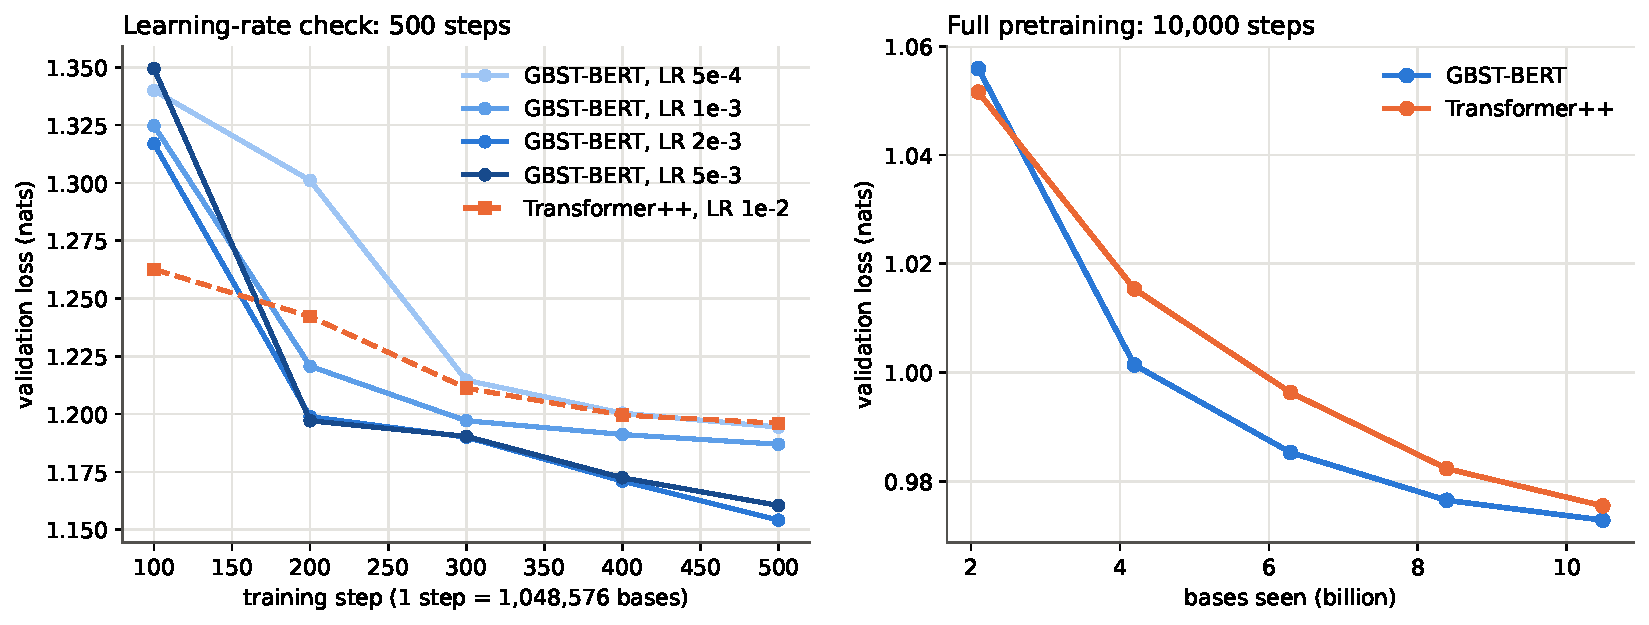
\includegraphics[width=\linewidth]{figures/pretraining_curves.pdf}
  \caption{Validation loss. Left: learning-rate search for GBST-BERT over 500 steps, with
  Transformer++ at its paper value. Right: full pretraining of both models.}
  \label{fig:pretrain}
\end{figure}

\begin{table}[t]
  \caption{Masked-base prediction on 2,048 unseen test sequences (311,767 masked bases, identical
  masks for both models).}
  \label{tab:pretrain}
  \centering
  \small
  \begin{tabular}{lcc}
    \toprule
    Model & Test loss (nats) & Accuracy \\
    \midrule
    GBST-BERT & \textbf{0.9753} & \textbf{56.44\%} \\
    Transformer++ & 0.9774 & 56.33\% \\
    Random guess & 1.3863 & 25.00\% \\
    Always the most common base & -- & 29.42\% \\
    \bottomrule
  \end{tabular}
\end{table}

Both models learn well beyond base composition (Table~\ref{tab:pretrain}). GBST-BERT is ahead on
validation loss for most of training (Figure~\ref{fig:pretrain}), but the final gap of 0.11 percentage
points cannot be interpreted with one run per model. Pretraining does not separate them.

\subsection{What GBST learned}\label{sec:gbstres}

We measure the share of GBST's weight on each block size, averaged over 8 hg38 sequences from
different chromosomes. For blocks of 1/2/3/4 bases it is 72/22/5/1\% after 500 steps at learning rate
$5\mathrm{e}{-4}$, but 98/2/0/0\% after 500 steps at $2\mathrm{e}{-3}$ and in the final model. GBST
therefore does \emph{not} learn multi-base units on human DNA under this setup: at the learning rate
we selected, it reads single bases almost exclusively. Each base has already been mixed with its
neighbours by the convolution, so the module acts mainly as a learned local filter. The early
difference between learning rates also shows that this outcome depends on training conditions.

\subsection{Nucleotide Transformer benchmark}

\begin{table}[t]
  \caption{NT benchmark test scores, mean $\pm$ range over 10 seeds. The first five columns are
  Bio-xLSTM Table 1; the last two are ours. Bold: best mean (ties counted for each model).}
  \label{tab:nt}
  \centering
  \scriptsize
  \setlength{\tabcolsep}{2.5pt}
  \resizebox{\linewidth}{!}{\begin{tabular}{lccccccc}
\toprule
Task & HyenaDNA & Mamba-PS & Mamba-PH & xLSTM-PS & xLSTM-PH & GBST-BERT & Transformer++ \\
\midrule
\multicolumn{8}{l}{\emph{Histone marks (MCC)}} \\
H3 & 0.779{\scriptsize$\,\pm\,$0.037} & 0.799{\scriptsize$\,\pm\,$0.029} & 0.815{\scriptsize$\,\pm\,$0.048} & 0.796{\scriptsize$\,\pm\,$0.014} & \textbf{0.824{\scriptsize$\,\pm\,$0.010}} & 0.815{\scriptsize$\,\pm\,$0.031} & 0.801{\scriptsize$\,\pm\,$0.029} \\
H3K14ac & 0.612{\scriptsize$\,\pm\,$0.065} & 0.541{\scriptsize$\,\pm\,$0.212} & 0.631{\scriptsize$\,\pm\,$0.026} & 0.570{\scriptsize$\,\pm\,$0.008} & 0.598{\scriptsize$\,\pm\,$0.017} & \textbf{0.673{\scriptsize$\,\pm\,$0.016}} & 0.569{\scriptsize$\,\pm\,$0.062} \\
H3K36me3 & 0.613{\scriptsize$\,\pm\,$0.041} & 0.609{\scriptsize$\,\pm\,$0.109} & 0.601{\scriptsize$\,\pm\,$0.129} & 0.588{\scriptsize$\,\pm\,$0.019} & 0.625{\scriptsize$\,\pm\,$0.010} & \textbf{0.655{\scriptsize$\,\pm\,$0.035}} & 0.591{\scriptsize$\,\pm\,$0.032} \\
H3K4me1 & 0.512{\scriptsize$\,\pm\,$0.024} & 0.488{\scriptsize$\,\pm\,$0.102} & 0.523{\scriptsize$\,\pm\,$0.039} & 0.490{\scriptsize$\,\pm\,$0.012} & 0.526{\scriptsize$\,\pm\,$0.001} & \textbf{0.565{\scriptsize$\,\pm\,$0.038}} & 0.481{\scriptsize$\,\pm\,$0.037} \\
H3K4me2 & 0.455{\scriptsize$\,\pm\,$0.095} & 0.388{\scriptsize$\,\pm\,$0.101} & 0.487{\scriptsize$\,\pm\,$0.170} & 0.489{\scriptsize$\,\pm\,$0.024} & 0.504{\scriptsize$\,\pm\,$0.012} & \textbf{0.509{\scriptsize$\,\pm\,$0.212}} & 0.367{\scriptsize$\,\pm\,$0.076} \\
H3K4me3 & 0.549{\scriptsize$\,\pm\,$0.056} & 0.440{\scriptsize$\,\pm\,$0.202} & 0.544{\scriptsize$\,\pm\,$0.045} & 0.520{\scriptsize$\,\pm\,$0.019} & 0.537{\scriptsize$\,\pm\,$0.012} & \textbf{0.553{\scriptsize$\,\pm\,$0.180}} & 0.362{\scriptsize$\,\pm\,$0.219} \\
H3K79me3 & 0.672{\scriptsize$\,\pm\,$0.048} & 0.676{\scriptsize$\,\pm\,$0.026} & \textbf{0.697{\scriptsize$\,\pm\,$0.077}} & 0.662{\scriptsize$\,\pm\,$0.011} & \textbf{0.697{\scriptsize$\,\pm\,$0.007}} & \textbf{0.697{\scriptsize$\,\pm\,$0.132}} & 0.676{\scriptsize$\,\pm\,$0.041} \\
H3K9ac & 0.581{\scriptsize$\,\pm\,$0.061} & 0.604{\scriptsize$\,\pm\,$0.048} & 0.622{\scriptsize$\,\pm\,$0.030} & 0.622{\scriptsize$\,\pm\,$0.013} & 0.627{\scriptsize$\,\pm\,$0.008} & \textbf{0.648{\scriptsize$\,\pm\,$0.037}} & 0.599{\scriptsize$\,\pm\,$0.046} \\
H4 & 0.763{\scriptsize$\,\pm\,$0.044} & 0.789{\scriptsize$\,\pm\,$0.020} & 0.811{\scriptsize$\,\pm\,$0.022} & 0.793{\scriptsize$\,\pm\,$0.011} & \textbf{0.813{\scriptsize$\,\pm\,$0.008}} & 0.804{\scriptsize$\,\pm\,$0.074} & 0.803{\scriptsize$\,\pm\,$0.022} \\
H4ac & 0.564{\scriptsize$\,\pm\,$0.038} & 0.525{\scriptsize$\,\pm\,$0.240} & 0.621{\scriptsize$\,\pm\,$0.054} & 0.558{\scriptsize$\,\pm\,$0.018} & 0.583{\scriptsize$\,\pm\,$0.014} & \textbf{0.642{\scriptsize$\,\pm\,$0.037}} & 0.528{\scriptsize$\,\pm\,$0.036} \\
\multicolumn{8}{l}{\emph{Enhancers (MCC)}} \\
enhancers & 0.517{\scriptsize$\,\pm\,$0.117} & 0.491{\scriptsize$\,\pm\,$0.066} & \textbf{0.546{\scriptsize$\,\pm\,$0.073}} & 0.375{\scriptsize$\,\pm\,$0.030} & 0.545{\scriptsize$\,\pm\,$0.024} & 0.336{\scriptsize$\,\pm\,$0.085} & 0.368{\scriptsize$\,\pm\,$0.074} \\
enhancers\_types & 0.386{\scriptsize$\,\pm\,$0.185} & 0.416{\scriptsize$\,\pm\,$0.095} & 0.439{\scriptsize$\,\pm\,$0.054} & 0.444{\scriptsize$\,\pm\,$0.046} & \textbf{0.466{\scriptsize$\,\pm\,$0.011}} & 0.430{\scriptsize$\,\pm\,$0.167} & 0.384{\scriptsize$\,\pm\,$0.053} \\
\multicolumn{8}{l}{\emph{Promoters (F1)}} \\
promoter\_all & 0.960{\scriptsize$\,\pm\,$0.005} & 0.967{\scriptsize$\,\pm\,$0.004} & 0.970{\scriptsize$\,\pm\,$0.004} & 0.962{\scriptsize$\,\pm\,$0.002} & 0.967{\scriptsize$\,\pm\,$0.001} & \textbf{0.971{\scriptsize$\,\pm\,$0.003}} & 0.968{\scriptsize$\,\pm\,$0.006} \\
promoter\_no\_tata & 0.959{\scriptsize$\,\pm\,$0.011} & 0.968{\scriptsize$\,\pm\,$0.006} & 0.968{\scriptsize$\,\pm\,$0.010} & 0.963{\scriptsize$\,\pm\,$0.002} & 0.970{\scriptsize$\,\pm\,$0.001} & \textbf{0.972{\scriptsize$\,\pm\,$0.006}} & 0.969{\scriptsize$\,\pm\,$0.004} \\
promoter\_tata & 0.944{\scriptsize$\,\pm\,$0.040} & \textbf{0.957{\scriptsize$\,\pm\,$0.015}} & 0.953{\scriptsize$\,\pm\,$0.016} & 0.948{\scriptsize$\,\pm\,$0.006} & 0.952{\scriptsize$\,\pm\,$0.005} & 0.948{\scriptsize$\,\pm\,$0.021} & 0.953{\scriptsize$\,\pm\,$0.013} \\
\multicolumn{8}{l}{\emph{Splice sites (accuracy / F1)}} \\
splice\_sites\_all & 0.956{\scriptsize$\,\pm\,$0.011} & 0.927{\scriptsize$\,\pm\,$0.021} & 0.940{\scriptsize$\,\pm\,$0.027} & 0.965{\scriptsize$\,\pm\,$0.006} & 0.974{\scriptsize$\,\pm\,$0.004} & \textbf{0.980{\scriptsize$\,\pm\,$0.004}} & 0.975{\scriptsize$\,\pm\,$0.006} \\
splice\_sites\_acceptors & 0.958{\scriptsize$\,\pm\,$0.010} & 0.936{\scriptsize$\,\pm\,$0.077} & 0.937{\scriptsize$\,\pm\,$0.033} & 0.970{\scriptsize$\,\pm\,$0.005} & 0.953{\scriptsize$\,\pm\,$0.008} & \textbf{0.977{\scriptsize$\,\pm\,$0.009}} & 0.955{\scriptsize$\,\pm\,$0.049} \\
splice\_sites\_donors & 0.949{\scriptsize$\,\pm\,$0.024} & 0.874{\scriptsize$\,\pm\,$0.289} & 0.948{\scriptsize$\,\pm\,$0.025} & 0.962{\scriptsize$\,\pm\,$0.004} & 0.951{\scriptsize$\,\pm\,$0.005} & \textbf{0.980{\scriptsize$\,\pm\,$0.012}} & 0.909{\scriptsize$\,\pm\,$0.117} \\
\midrule
Tasks with the best mean & 0 & 1 & 2 & 0 & 4 & 13 & 0 \\
\bottomrule
\end{tabular}
}
\end{table}

GBST-BERT has the best mean on 13 of 18 tasks (Table~\ref{tab:nt}; xLSTM-PH 4, Mamba-PH 2, Mamba-PS 1,
Transformer++ 0). It exceeds Transformer++ on 16 of 18 tasks (two-sided sign test over tasks
$p=0.0013$; the tasks are related, so this value is only a guide). The largest gains are on histone
marks (e.g.\ H3K4me3 $+0.190$, H3K4me2 $+0.142$, H4ac $+0.114$ MCC) and on splice donors ($+0.071$
F1), while promoters differ by at most 0.005. Compared with the best paper model per task, GBST-BERT
is higher on 12 tasks and tied on one. The splice tasks received an extra learning-rate check, which the
paper's models did not need. Some GBST-BERT
ranges are wide (H3K4me2 $\pm0.212$, H3K4me3 $\pm0.180$), so single runs are unreliable on these tasks.

\subsection{Why the enhancer tasks are weak}\label{sec:enh}

\begin{table}[t]
  \caption{Validation and test scores (MCC). Our models: mean over 10 seeds. 4-mer baseline: logistic
  regression on 4-mer frequencies, one 90/10 split. Last column: test sequences with an exact copy in
  the training file. Copies always carry the same label.}
  \label{tab:enh}
  \centering
  \small
  \setlength{\tabcolsep}{4pt}
  \resizebox{\linewidth}{!}{\begin{tabular}{lcccccccc}
\toprule
& \multicolumn{2}{c}{GBST-BERT} & \multicolumn{2}{c}{Transformer++} & \multicolumn{3}{c}{4-mer logistic regression} & Test seqs. \\
\cmidrule(lr){2-3}\cmidrule(lr){4-5}\cmidrule(lr){6-8}
Task & val. & test & val. & test & val. & test & test, no copies & in train \\
\midrule
enhancers & 0.871 & 0.336 & 0.899 & 0.368 & 0.794 & 0.436 & 0.319 & 100/400 \\
enhancers\_types & 0.789 & 0.430 & 0.788 & 0.384 & 0.777 & 0.299 & 0.168 & 100/400 \\
promoter\_all & 0.973 & 0.971 & 0.970 & 0.968 & 0.807 & 0.802 & 0.802 & 21/5920 \\
H3 & 0.811 & 0.815 & 0.787 & 0.801 & 0.634 & 0.631 & 0.631 & 0/1497 \\
\bottomrule
\end{tabular}
}
\end{table}

Enhancers are the clear weakness: MCC 0.336 against 0.546 for the best paper model. Our logs show that
these two tasks stand apart: validation scores far exceed test scores (gap 0.53 and 0.36 for
GBST-BERT), while on the 16 other tasks the gap never exceeds 0.05. Transformer++ behaves the same
way, so GBST is not the cause.

To test whether this is a modelling problem at all, we trained a plain logistic regression on 4-mer
frequencies, with no neural network and no pretraining (Table~\ref{tab:enh}). It shows the same drop
on the enhancer tasks (0.79 to 0.44, and 0.78 to 0.30) and none on the controls. The gap is therefore
a property of the dataset: what separates the classes in the training file transfers only partly to
the test file. On the binary task this simple baseline even exceeds both of our models on test,
which suggests that they fit training-specific patterns more closely than a 4-mer model can.

Two further points affect how these tasks should be read. First, 100 of the 400 test sequences are
exact copies of training sequences, so the test score partly measures recall; the baseline's score
falls further when they are removed. Second, validation scores cannot guide model selection here, as
they do not reflect test behaviour. We did not determine why some published models reach higher test
scores on these tasks; with 400 test sequences the estimates are also noisy.

\section{Discussion and limitations}\label{sec:disc}

\textbf{Answers to the research questions.} \emph{RQ1:} GBST does not measurably improve masked-base
prediction; the final difference of 0.11 percentage points is too small to interpret with one run per
model. \emph{RQ2:} on the NT benchmark GBST-BERT is ahead of its control on 16 of 18 tasks and has the
best mean of seven models on 13.
\emph{RQ3:} GBST does not form multi-base units; it settles on single bases.

\textbf{Where the gains appear.} The NT gains are uneven. GBST-BERT has the best mean on 8 of 10 histone
tasks and on all 3 splice tasks, and the differences from the control are largest on histone marks.
Promoter scores are close to their ceiling for every model, so these tasks separate models little.
Both groups with large gains may depend on sequence patterns that a short filter can capture, which
would be compatible with a role for the convolution, but we have not tested this link.

\textbf{Pretraining loss did not predict downstream behaviour.} The two models are nearly identical in
masked-base prediction, yet they differ strongly on several downstream tasks. Pretraining loss alone
would therefore have hidden the differences reported here. One possible reason is that the loss
averages over all bases, most of which carry little task-relevant signal, whereas each task depends on
specific patterns. This suggests evaluating small DNA models on downstream tasks as well as on loss.

\textbf{Why GBST may prefer single bases.} We can offer hypotheses only. MLM asks for one base at each
position, which may favour the block that keeps that position's identity most directly. Because masking
acts on the input, longer blocks around a masked base also mix in the \texttt{[MASK]} token. The outcome
also depends on training conditions: after 500 steps, the weight on single bases was 72\% at learning
rate $5\mathrm{e}{-4}$ and 98\% at $2\mathrm{e}{-3}$. As we selected the learning rate by validation
loss, the better-predicting of these two settings is also the one that uses longer blocks less. Whether GBST
would use longer blocks with another objective, a longer context or downsampling remains open.

\textbf{Training stability.} GBST-BERT is not uniformly more robust. It collapsed to one class on splice
tasks at the paper's learning rates, and some histone tasks show wide ranges between seeds. Transformer++
shows such ranges as well, for example on splice donors ($\pm0.117$). Mean scores should therefore be
read together with their ranges, and single runs can mislead on these tasks.

\textbf{What the enhancer result means for benchmarking.} The diagnosis in Section~\ref{sec:enh} applies
to any model evaluated on these two tasks, including published ones. High validation scores are not
evidence of good test performance here, duplicated sequences inflate test scores, and with 400 test
sequences small differences are unreliable. Our analysis does not show that these tasks are unusable,
and it does not explain why some models score higher on them.

\textbf{What cannot be claimed yet.} We have not shown that \emph{tokenization} causes the gain. GBST
reads single bases, so learned multi-base units cannot explain it. We suspect the convolution, but this
is a hypothesis. The two models also differ in normalization and in how their pretraining learning rate
was chosen, and either difference could contribute. The comparison with published models is also
limited: they were tuned per model, while we reused settings chosen for DNA-xLSTM-PH.

\textbf{Further limitations.}
\begin{itemize}
  \item \emph{One pretraining run per model.} Variation from pretraining is unmeasured, and the
  fine-tuning repeats capture only part of the uncertainty.
  \item \emph{Unequal data exposure.} A data-loader bug corrupted 0.35\% of sequences during GBST-BERT's
  first 3,000 steps. Corrupted reads stayed within their data split. Transformer++ was trained after the
  fix, so only GBST-BERT saw this data.
  \item \emph{Reading of ChaRNABERT.} We added a pointwise layer inferred from its parameter table, used
  blocks that contain each position, used standard SwiGLU, and chose the maximum block size of 4
  ourselves. A different reading could change the results.
  \item \emph{Fine-tuning details.} Settings came from another architecture and were tuned only on splice
  tasks. This applies equally to both of our models.
  \item \emph{Scope.} We tested one model size, one context length and classification tasks only.
  Nothing here supports clinical use.
\end{itemize}

\section{Conclusion}

We transferred ChaRNABERT's learned tokenizer to human DNA at the 2M-parameter scale of DNA-xLSTM and
compared it with a same-shape control in pretraining and on 18 downstream tasks. Three findings stand
out. First, GBST-BERT is a competitive small DNA model: it has the best mean of seven models on 13 of 18
NT tasks, and it exceeds its control on 16 of them. Second, the tokenizer did not
behave as motivated: it chose single bases and formed no multi-base units, so the improvement, if it
comes from GBST at all, must have another source. Third, the weak enhancer scores coincide with a
train--test mismatch and duplicated sequences in the benchmark, which matters for anyone comparing
models on these two tasks.

The most useful next experiments follow directly from these findings:
\begin{enumerate}
  \item \emph{Ablation of GBST.} Train the same model with an embedding table instead of GBST. If it
  matches GBST-BERT, the gain comes from normalization or tuning rather than from GBST.
  \item \emph{Convolution only.} Keep the convolution and remove the block selection. If this variant
  matches GBST-BERT, local mixing explains the gain, and a much simpler module would be enough.
  \item \emph{Repeated pretraining.} Pretrain each model with several seeds to measure the variation
  that is currently unknown.
  \item \emph{Conditions that favour longer blocks.} Test other learning rates, longer contexts and
  other objectives such as UL2, which the code already supports.
  \item \emph{Fairer fine-tuning.} Run the same hyperparameter search for our models as the paper ran
  for its own.
  \item \emph{Cleaner enhancer evaluation.} Remove duplicates and build a validation set that reflects
  the test distribution.
\end{enumerate}

The practical lesson of this work is that a good benchmark score does not by itself explain what a model
has learned. Looking inside the model and at the data changed both of the interpretations we started
with: that GBST learns useful DNA units, and that weak enhancer scores are a modelling problem.

\section*{Code and reproducibility}

{\raggedright
\begin{itemize}
  \item Repository (branch \texttt{charna-gbst}):\\ {\small\url{\repo}}
  \item Full notebook, executed, with every step, table and figure:\\
  {\small\url{\notebook}}
  \item Fine-tuned NT models:\\ {\small\url{\repo/releases/tag/nt-finetuned-models}}
\end{itemize}
}

The notebook re-computes the data statistics, the final test of both pretrained models, the GBST
analysis, all tables and figures, the enhancer diagnosis, and one fine-tuning job per benchmark. It
loads the saved results of the original pretraining and fine-tuning runs; setting its switches
to \texttt{True} repeats those long runs with the same scripts.

\bibliographystyle{plainnat}
\bibliography{refs}

\clearpage
\appendix

\section{Settings}\label{app:hparams}

Table~\ref{tab:settings} lists the main settings and their sources.

\begin{center}
  \small
  \captionof{table}{Main settings and their sources.}\label{tab:settings}
  \begin{tabularx}{\linewidth}{lX}
    \toprule
    Model & 256 dimensions, 4 blocks, 8 heads, SwiGLU hidden size 320, no norm or linear biases [Bio-xLSTM Table A3] \\
    GBST & blocks of 1--4 bases with offsets, sum pooling, calibration, no downsampling [ChaRNABERT Sec.~3.2]; maximum block size 4 is our choice \\
    Masking & 15\% of positions; 80\% \texttt{[MASK]}, 10\% random, 10\% unchanged [Bio-xLSTM App.~C.5] \\
    Batch & 1,024 sequences of 1,024 bases per step [Bio-xLSTM App.~C.5] \\
    Optimizer & AdamW, $\beta=(0.9,0.95)$, weight decay 0.1, 10\% warm-up, cosine decay [Bio-xLSTM Table A4] \\
    Learning rate & GBST-BERT $2\mathrm{e}{-3}$ (our search); Transformer++ $1\mathrm{e}{-2}$ [Bio-xLSTM Table A3] \\
    Precision & 32-bit; our GPUs (GTX 1080 Ti, RTX 2080 Ti, Quadro GV100) have no bf16 \\
    \bottomrule
  \end{tabularx}
\end{center}

\section{Tasks}\label{app:tasks}

\begin{center}
  \small
  \captionof{table}{The 18 NT tasks. Learning rate and batch size: Bio-xLSTM Table A5, DNA-xLSTM-PH column.}
  \resizebox{\linewidth}{!}{\begin{tabular}{llcrrrlcc}
\toprule
Task & Group & Classes & Length & Train & Test & Score & LR & Batch \\
\midrule
H3 & histone mark & 2 & 500 & 13,468 & 1,497 & MCC & 8e-4 & 128 \\
H3K14ac & histone mark & 2 & 500 & 29,743 & 3,305 & MCC & 6e-4 & 128 \\
H3K36me3 & histone mark & 2 & 500 & 31,392 & 3,488 & MCC & 6e-4 & 64 \\
H3K4me1 & histone mark & 2 & 500 & 28,509 & 3,168 & MCC & 8e-4 & 128 \\
H3K4me2 & histone mark & 2 & 500 & 27,614 & 3,069 & MCC & 6e-4 & 64 \\
H3K4me3 & histone mark & 2 & 500 & 33,119 & 3,680 & MCC & 8e-4 & 128 \\
H3K79me3 & histone mark & 2 & 500 & 25,953 & 2,884 & MCC & 1e-3 & 128 \\
H3K9ac & histone mark & 2 & 500 & 25,003 & 2,779 & MCC & 4e-4 & 64 \\
H4 & histone mark & 2 & 500 & 13,140 & 1,461 & MCC & 8e-4 & 64 \\
H4ac & histone mark & 2 & 500 & 30,685 & 3,410 & MCC & 4e-4 & 64 \\
enhancers & enhancer & 2 & 200 & 14,968 & 400 & MCC & 2e-3 & 512 \\
enhancers\_types & enhancer & 3 & 200 & 14,968 & 400 & MCC & 2e-3 & 512 \\
promoter\_all & promoter & 2 & 300 & 53,276 & 5,920 & F1 & 4e-4 & 64 \\
promoter\_no\_tata & promoter & 2 & 300 & 47,767 & 5,299 & F1 & 1e-3 & 128 \\
promoter\_tata & promoter & 2 & 300 & 5,509 & 621 & F1 & 3e-3 & 128 \\
splice\_sites\_all & splice site & 3 & 400 & 27,000 & 3,000 & accuracy & 8e-4 & 64 \\
splice\_sites\_acceptors & splice site & 2 & 600 & 19,961 & 2,218 & F1 & 2e-3 & 128 \\
splice\_sites\_donors & splice site & 2 & 600 & 19,775 & 2,198 & F1 & 3e-3 & 128 \\
\bottomrule
\end{tabular}
}
\end{center}

\end{document}
